%%
%%  Annexes
%%
%%  Note: Ne pas modifier la ligne ci-dessous. / Do not modify the following line.
\ifthenelse{\equal{\Langue}{english}}{
	\addcontentsline{toc}{compteur}{APPENDICES}
}{
	\addcontentsline{toc}{compteur}{ANNEXES}
}
%%
%%
%%  Toutes les annexes doivent être inclues dans ce document
%%  les unes à la suite des autres.
%%  All annexes must be included in this document one after the other.
% \Annexe{Démo}
% Texte de l'annexe B\@. Remarquez que la phrase précédente se termine
% par une lettre majuscule suivie d'un point. On indique explicitement
% cette situation à \LaTeX{} afin que ce dernier ajuste correctement
% l'espacement entre le point final de la phrase et le début de la
% phrase suivante.
% une autre page!


% \begin{landscape}
% \Annexe{Encore une annexe / Another Appendix}
% Texte de l'annexe B\@ en mode «landscape».
% \end{landscape}

% \Annexe{Une dernière annexe / The Last Appendix}
% Texte de l'annexe C\@.

\Annexe{Méthodologie revue de littérature et développement Agile} \label{annexe_methodologie}

\begin{figure}[htb]
\centering
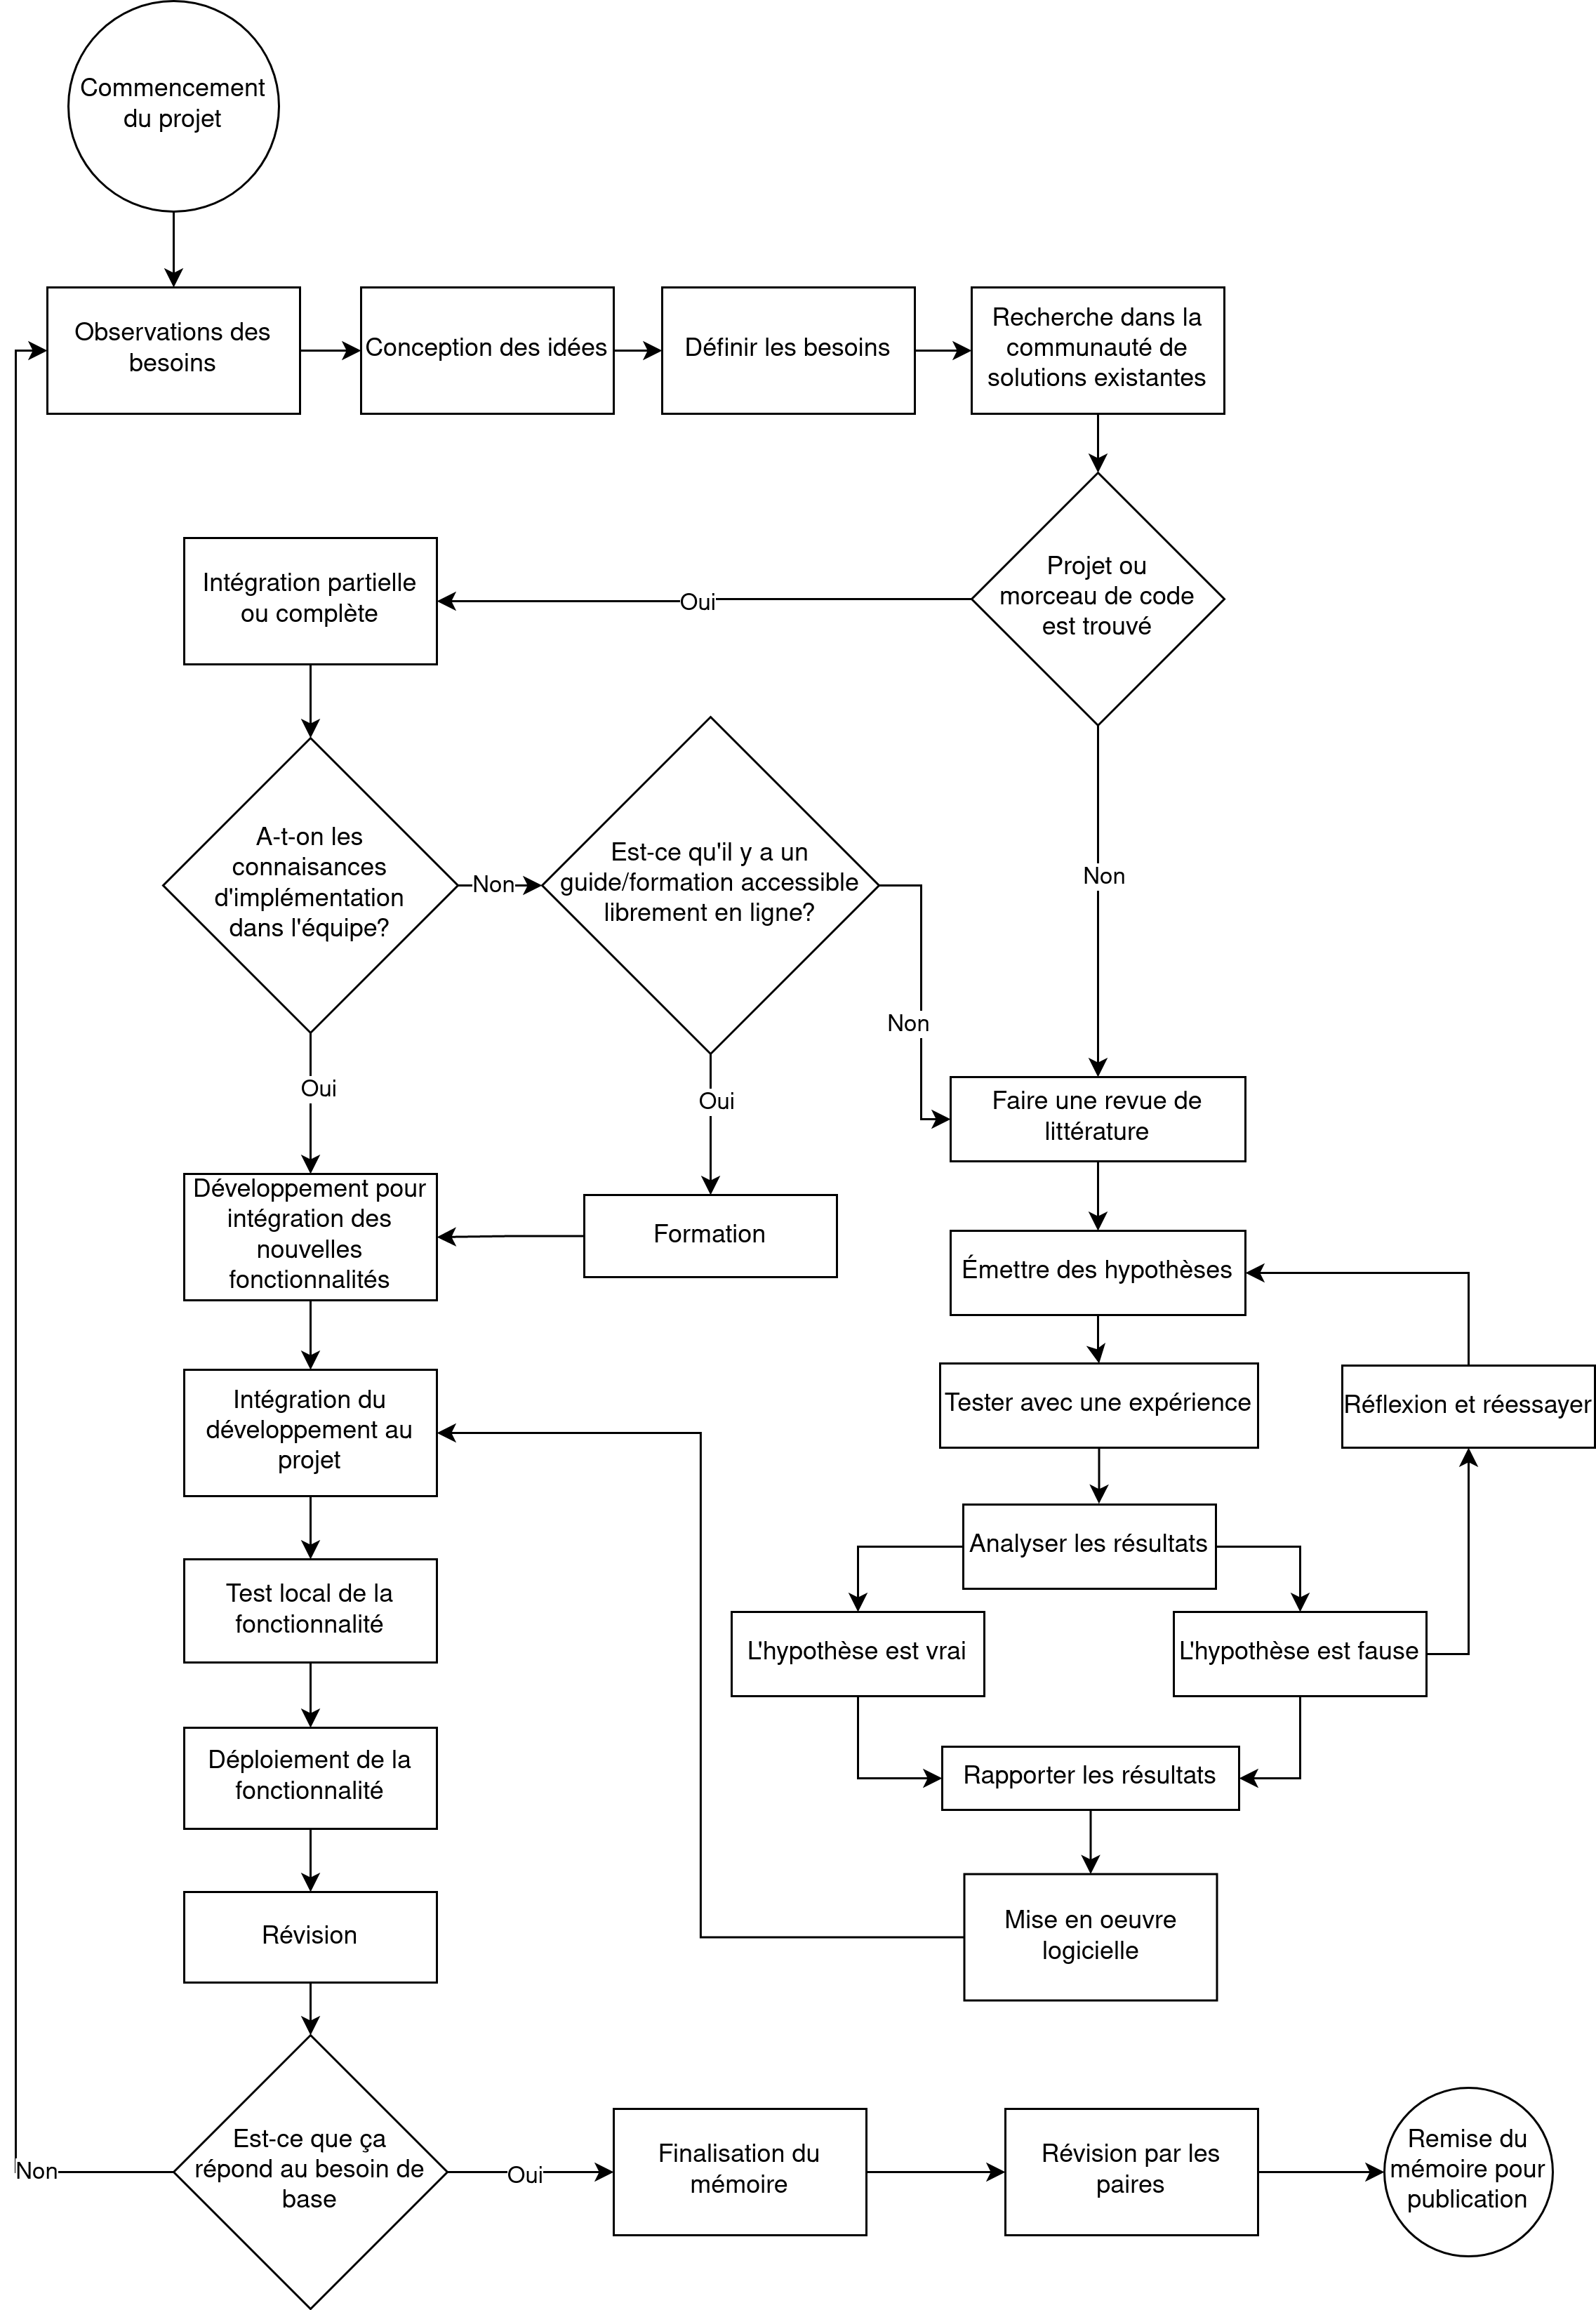
\includegraphics[height=7in]{images/methodologie_scientifique.drawio.png}
\end{figure}

\Annexe{GUI générateur de code - les modèles} \label{annexe_cg_gui_model}

\begin{figure}[htb]
\centering
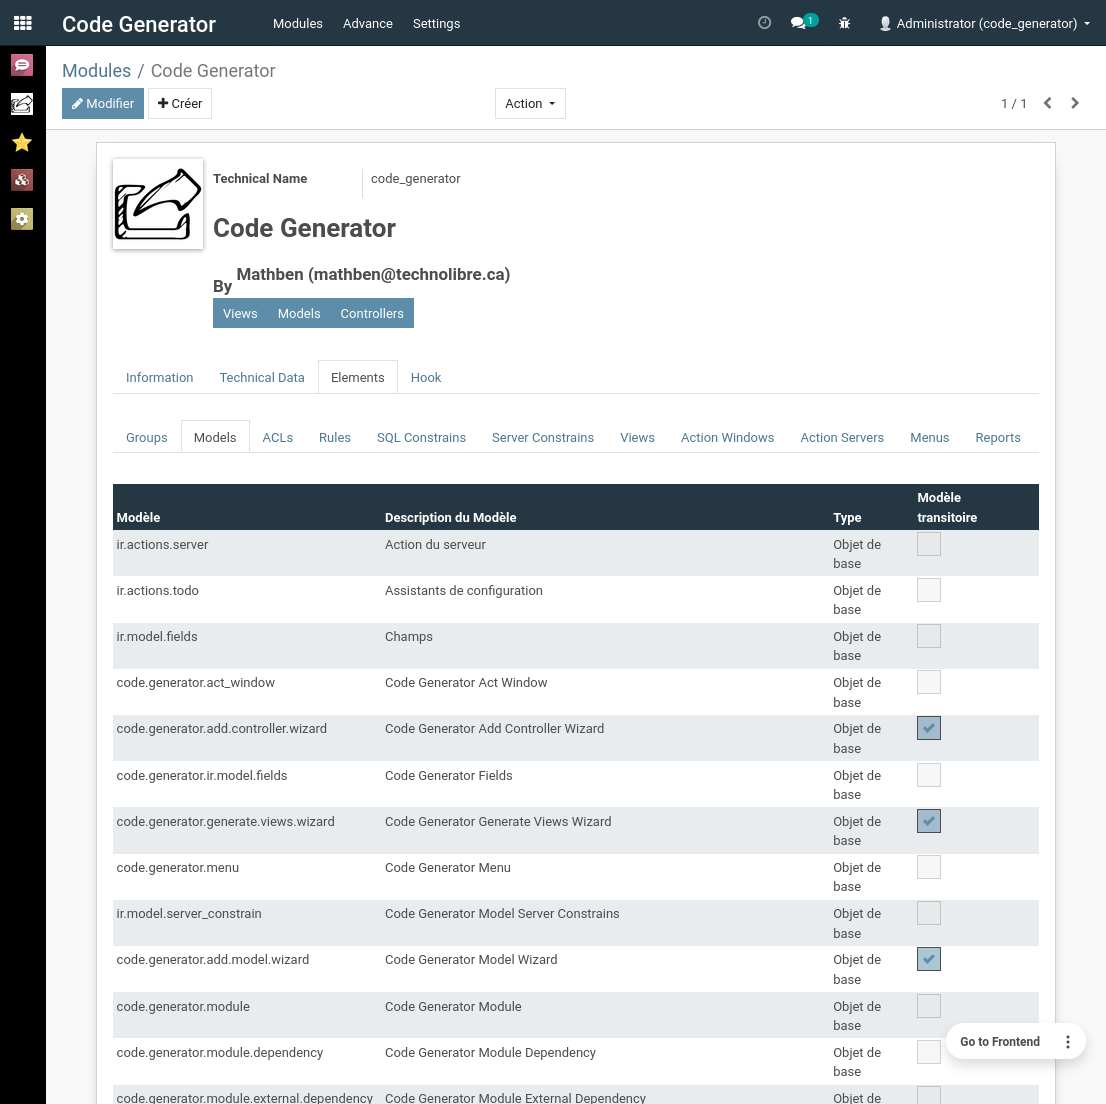
\includegraphics[width=\textwidth]{cg_model.png}
\end{figure}

\Annexe{GUI générateur de code - les champs} \label{annexe_cg_gui_champs}

\begin{figure}[htb]
\centering
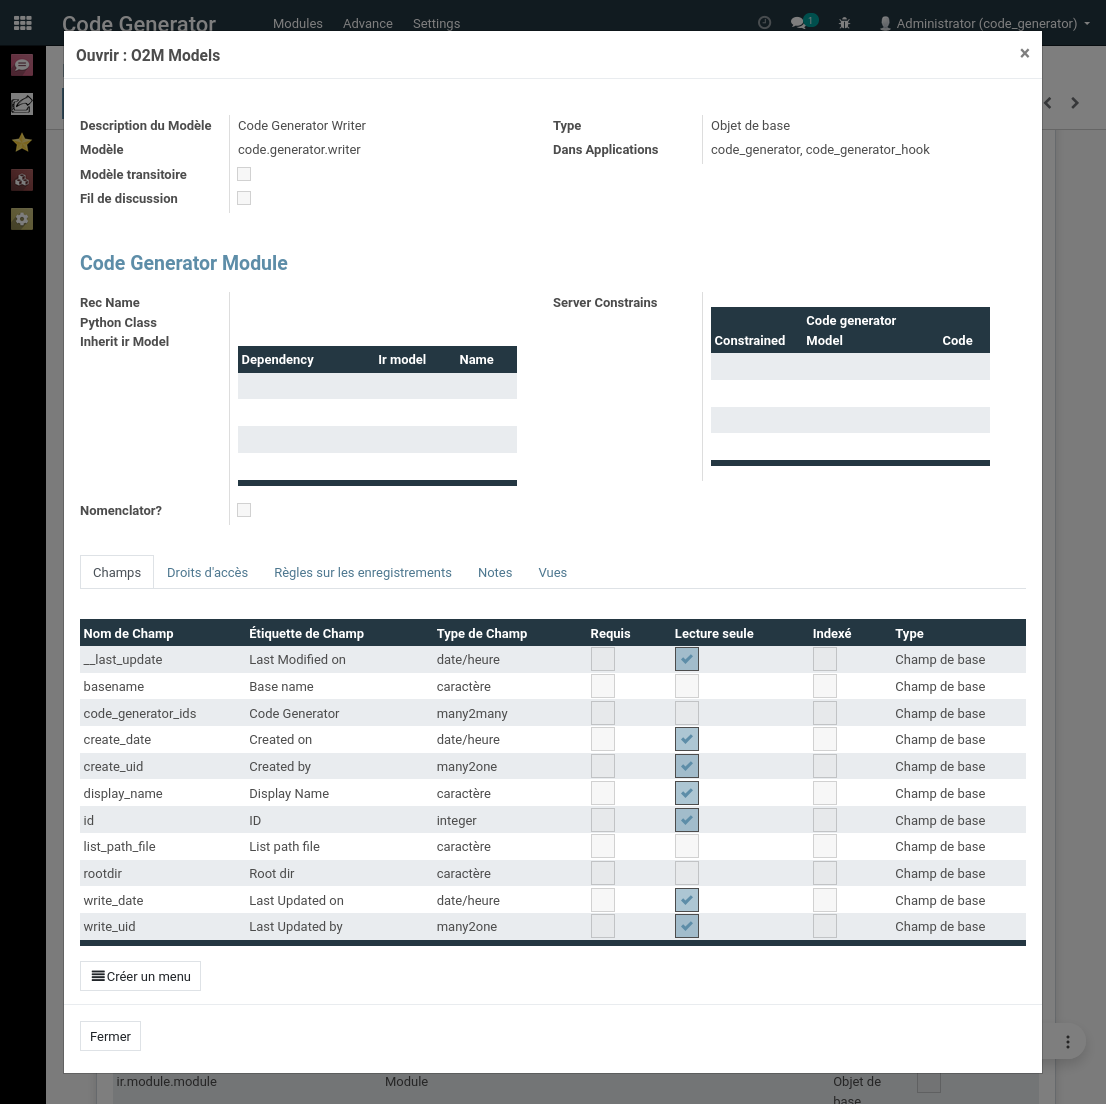
\includegraphics[width=\textwidth]{cg_champs.png}
\end{figure}

\Annexe{GUI générateur de code - les codes} \label{annexe_cg_gui_code}

\begin{figure}[htb]
\centering
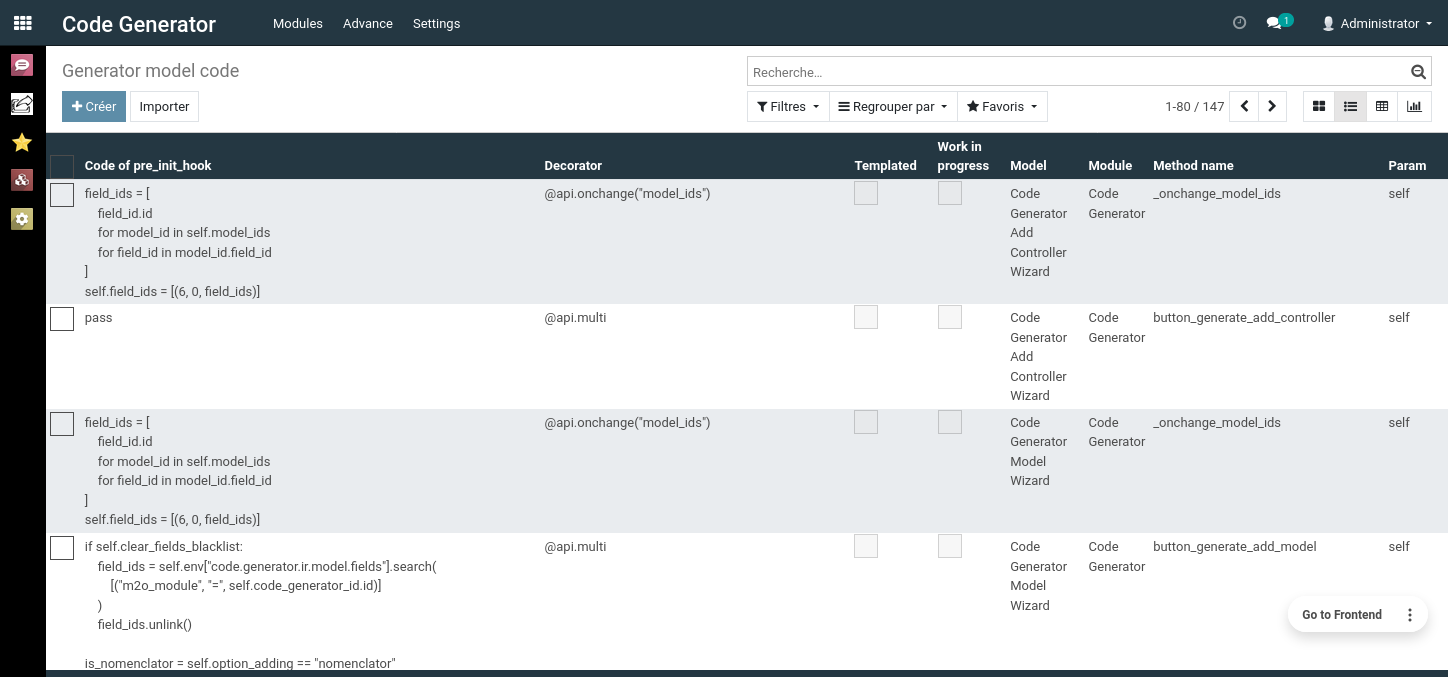
\includegraphics[width=\textwidth]{cg_code.png}
\end{figure}

\Annexe{GUI générateur de code - les «hooks»} \label{annexe_cg_gui_hook}

\begin{figure}[htb]
\centering
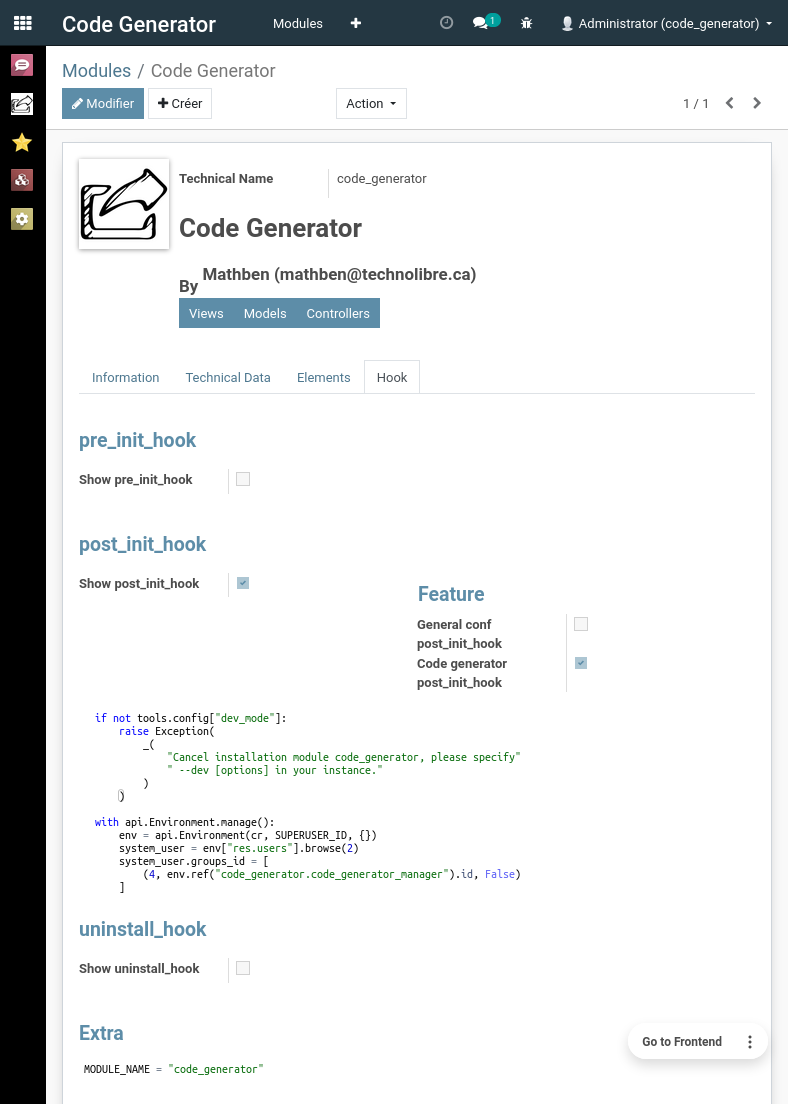
\includegraphics[height=7in]{cg_hook.png}
\end{figure}


\Annexe{Test couverture technique générateur de code} \label{annexe_test_generateur_code}

\begin{table}[htb]
\centering
\begin{tabular}{|l|l|l|l|l|l|}

\hline
\cellcolor[HTML]{d9d9d9}{\textbf{Technique}} & \multicolumn{2}{|l|}{\cellcolor[HTML]{d9d9d9}{base}} & \multicolumn{2}{|l|}{\cellcolor[HTML]{d9d9d9}{\textbf{\# instruction}}} & \cellcolor[HTML]{d9d9d9}{5 085}\\\hline

\multicolumn{2}{|l|}{\cellcolor[HTML]{efefef}{\textbf{Description du test}}} & \cellcolor[HTML]{efefef}{\textbf{Status}} & \cellcolor[HTML]{efefef}{\textbf{Durée (s)}} & \cellcolor[HTML]{efefef}{\textbf{\# de Miss}} & \cellcolor[HTML]{efefef}{\textbf{Cover (\%)}}\\\hline

\multicolumn{2}{|l|}{\shortstack[l]{Génération µ$_C^B$ modèle simple}} & Succès & 27 & 2 983 & 41\\\hline

\multicolumn{2}{|l|}{\shortstack[l]{Génération µ$_C^B$ modèle simple avec \\ héritage}} & Succès & 26 & 3 452 & 32\\\hline

\multicolumn{2}{|l|}{\shortstack[l]{Exportation µ$_C^B$ données «helpdesk»}} & Succès & 28 & 3 900 & 23\\\hline

% \end{tabular}
% \end{table}
% \begin{table}
% \centering
% \begin{tabular}{|l|l|l|l|l|l|}
% \hline

\cellcolor[HTML]{d9d9d9}{\textbf{Technique}} & \multicolumn{2}{|l|}{\cellcolor[HTML]{d9d9d9}{base + hook}} & \multicolumn{2}{|l|}{\cellcolor[HTML]{d9d9d9}{\textbf{\# instruction}}} & \cellcolor[HTML]{d9d9d9}{5 985}\\\hline

\multicolumn{2}{|l|}{\cellcolor[HTML]{efefef}{\textbf{Description du test}}} & \cellcolor[HTML]{efefef}{\textbf{Status}} & \cellcolor[HTML]{efefef}{\textbf{Durée (s)}} & \cellcolor[HTML]{efefef}{\textbf{\# de Miss}} & \cellcolor[HTML]{efefef}{\textbf{Cover (\%)}}\\\hline

\multicolumn{2}{|l|}{\shortstack[l]{Auto-génération µ$_C^0$}} & Succès & 17 & 4 683 & 22\\\hline

\multicolumn{2}{|l|}{\shortstack[l]{Nouveau projet µ$_C^0$ µ$_C^A$ µ$_C^B$ \\ «Hello World»}} & Succès & 39 & 4 610 & 23\\\hline

\multicolumn{2}{|l|}{\shortstack[l]{Génération µ$_C^A$ portail}} & Succès & 44 & 3 638 & 39\\\hline

\multicolumn{2}{|l|}{\shortstack[l]{Génération µ$_C^A$ modèle simple}} & Succès & 33 & 3 982 & 33\\\hline

\multicolumn{2}{|l|}{\shortstack[l]{Génération µ$_C^A$ modèle simple avec \\ héritage}} & Succès & 32 & 4 027 & 33\\\hline

\multicolumn{2}{|l|}{\shortstack[l]{Exportation µ$_C^B$ données «website»}} & Succès & 28 & 3 900 & 23\\\hline

\multicolumn{2}{|l|}{\shortstack[l]{Génération µ$_C^B$ du générateur de \\ code}} & Échec & 20 & 3 529 & 41\\\hline

\multicolumn{2}{|l|}{\shortstack[l]{Génération µ$_C^A$ du générateur de \\ code}} & Échec & 29 & 3 690 & 38\\\hline

% \end{tabular}
% \end{table}
% \begin{table}
% \centering
% \begin{tabular}{|l|l|l|l|l|l|}
% \hline

\cellcolor[HTML]{d9d9d9}{\textbf{Technique}} & \multicolumn{2}{|l|}{\cellcolor[HTML]{d9d9d9}{base + cron}} & \multicolumn{2}{|l|}{\cellcolor[HTML]{d9d9d9}{\textbf{\# instruction}}} & \cellcolor[HTML]{d9d9d9}{6 153}\\\hline

\multicolumn{2}{|l|}{\cellcolor[HTML]{efefef}{\textbf{Description du test}}} & \cellcolor[HTML]{efefef}{\textbf{Status}} & \cellcolor[HTML]{efefef}{\textbf{Durée (s)}} & \cellcolor[HTML]{efefef}{\textbf{\# de Miss}} & \cellcolor[HTML]{efefef}{\textbf{Cover (\%)}}\\\hline

\multicolumn{2}{|l|}{\shortstack[l]{Génération µ$_C^A$ «auto\_backup»}} & Succès & 36 & 3 422 & 44\\\hline

% \end{tabular}
% \end{table}
% \begin{table}
% \centering
% \begin{tabular}{|l|l|l|l|l|l|}
% \hline

\cellcolor[HTML]{d9d9d9}{\textbf{Technique}} & \multicolumn{2}{|l|}{\cellcolor[HTML]{d9d9d9}{base + portal}} & \multicolumn{2}{|l|}{\cellcolor[HTML]{d9d9d9}{\textbf{\# instruction}}} & \cellcolor[HTML]{d9d9d9}{5 799}\\\hline

\multicolumn{2}{|l|}{\cellcolor[HTML]{efefef}{\textbf{Description du test}}} & \cellcolor[HTML]{efefef}{\textbf{Status}} & \cellcolor[HTML]{efefef}{\textbf{Durée (s)}} & \cellcolor[HTML]{efefef}{\textbf{\# de Miss}} & \cellcolor[HTML]{efefef}{\textbf{Cover (\%)}}\\\hline

\multicolumn{2}{|l|}{\shortstack[l]{Génération µ$_C^B$ exemple MariaDB \\ SQL}} & Succès & 80 & 3 104 & 46\\\hline

% \end{tabular}
% \end{table}
% \begin{table}
% \centering
% \begin{tabular}{|l|l|l|l|l|l|}
% \hline

\cellcolor[HTML]{d9d9d9}{\textbf{Technique}} & \multicolumn{2}{|l|}{\cellcolor[HTML]{d9d9d9}{base + «theme\_website»}} & \multicolumn{2}{|l|}{\cellcolor[HTML]{d9d9d9}{\textbf{\# instruction}}} & \cellcolor[HTML]{d9d9d9}{5 336}\\\hline

\multicolumn{2}{|l|}{\cellcolor[HTML]{efefef}{\textbf{Description du test}}} & \cellcolor[HTML]{efefef}{\textbf{Status}} & \cellcolor[HTML]{efefef}{\textbf{Durée (s)}} & \cellcolor[HTML]{efefef}{\textbf{\# de Miss}} & \cellcolor[HTML]{efefef}{\textbf{Cover (\%)}}\\\hline

\multicolumn{2}{|l|}{\shortstack[l]{Génération µ$_C^B$ thème «website»}} & Succès & 27 & 3 938 & 26\\\hline

% \end{tabular}
% \end{table}
% \begin{table}
% \centering
% \begin{tabular}{|l|l|l|l|l|l|}
% \hline

\cellcolor[HTML]{d9d9d9}{\textbf{Technique}} & \multicolumn{2}{|l|}{\cellcolor[HTML]{d9d9d9}{base + «website\_snippet»}} & \multicolumn{2}{|l|}{\cellcolor[HTML]{d9d9d9}{\textbf{\# instruction}}} & \cellcolor[HTML]{d9d9d9}{5 615}\\\hline

\multicolumn{2}{|l|}{\cellcolor[HTML]{efefef}{\textbf{Description du test}}} & \cellcolor[HTML]{efefef}{\textbf{Status}} & \cellcolor[HTML]{efefef}{\textbf{Durée (s)}} & \cellcolor[HTML]{efefef}{\textbf{\# de Miss}} & \cellcolor[HTML]{efefef}{\textbf{Cover (\%)}}\\\hline

\multicolumn{2}{|l|}{\shortstack[l]{Génération µ$_C^B$ individuel \\ «website\_snippet»}} & Succès & 26 & 4 284 & 24\\\hline

\end{tabular}
\end{table}
\begin{table}[htb]
\centering
\begin{tabular}{|l|l|l|l|l|l|}
\hline

\cellcolor[HTML]{d9d9d9}{\textbf{Technique}} & \multicolumn{2}{|l|}{\cellcolor[HTML]{d9d9d9}{\shortstack[l]{base + portal + \\ «website\_snippet»}}} & \multicolumn{2}{|l|}{\cellcolor[HTML]{d9d9d9}{\textbf{\# instruction}}} & \cellcolor[HTML]{d9d9d9}{6 329}\\\hline

\multicolumn{2}{|l|}{\cellcolor[HTML]{efefef}{\textbf{Description du test}}} & \cellcolor[HTML]{efefef}{\textbf{Status}} & \cellcolor[HTML]{efefef}{\textbf{Durée (s)}} & \cellcolor[HTML]{efefef}{\textbf{\# de Miss}} & \cellcolor[HTML]{efefef}{\textbf{Cover (\%)}}\\\hline

\multicolumn{2}{|l|}{\shortstack[l]{Génération µ$_C^B$ multiple \\ «website\_snippet»}} & Succès & 36 & 2 898 & 54\\\hline

\multicolumn{2}{|l|}{\shortstack[l]{Génération µ$_C^B$ portail}} & Succès & 34 & 3 173 & 50\\\hline

% \end{tabular}
% \end{table}
% \begin{table}
% \centering
% \begin{tabular}{|l|l|l|l|l|l|}
% \hline

\cellcolor[HTML]{d9d9d9}{\textbf{Technique}} & \multicolumn{2}{|l|}{\cellcolor[HTML]{d9d9d9}{base + portal + «Migration DB»}} & \multicolumn{2}{|l|}{\cellcolor[HTML]{d9d9d9}{\textbf{\# instruction}}} & \cellcolor[HTML]{d9d9d9}{6 559}\\\hline

\multicolumn{2}{|l|}{\cellcolor[HTML]{efefef}{\textbf{Description du test}}} & \cellcolor[HTML]{efefef}{\textbf{Status}} & \cellcolor[HTML]{efefef}{\textbf{Durée (s)}} & \cellcolor[HTML]{efefef}{\textbf{\# de Miss}} & \cellcolor[HTML]{efefef}{\textbf{Cover (\%)}}\\\hline

\multicolumn{2}{|l|}{\shortstack[l]{Génération migration MariaDB \\ SQL}} & Succès & 121 & 3 267 & 50\\\hline

% \end{tabular}
% \end{table}
% \begin{table}
% \centering
% \begin{tabular}{|l|l|l|l|l|l|}

\hline
\cellcolor[HTML]{d9d9d9}{\textbf{Technique}} & \multicolumn{2}{|l|}{\cellcolor[HTML]{d9d9d9}{base + hook + portal}} & \multicolumn{2}{|l|}{\cellcolor[HTML]{d9d9d9}{\textbf{\# instruction}}} & \cellcolor[HTML]{d9d9d9}{6 699}\\\hline

\multicolumn{2}{|l|}{\cellcolor[HTML]{efefef}{\textbf{Description du test}}} & \cellcolor[HTML]{efefef}{\textbf{Status}} & \cellcolor[HTML]{efefef}{\textbf{Durée (s)}} & \cellcolor[HTML]{efefef}{\textbf{\# de Miss}} & \cellcolor[HTML]{efefef}{\textbf{Cover (\%)}}\\\hline

\multicolumn{2}{|l|}{\shortstack[l]{Génération µ$_C^A$ MariaDB SQL}} & Succès & 78 & 4 315 & 36\\\hline

% \end{tabular}
% \end{table}
% \begin{table}
% \centering
% \begin{tabular}{|l|l|l|l|l|l|}
% \hline

\cellcolor[HTML]{d9d9d9}{\textbf{Technique}} & \multicolumn{2}{|l|}{\cellcolor[HTML]{d9d9d9}{base + hook + cron}} & \multicolumn{2}{|l|}{\cellcolor[HTML]{d9d9d9}{\textbf{\# instruction}}} & \cellcolor[HTML]{d9d9d9}{6 153}\\\hline

\multicolumn{2}{|l|}{\cellcolor[HTML]{efefef}{\textbf{Description du test}}} & \cellcolor[HTML]{efefef}{\textbf{Status}} & \cellcolor[HTML]{efefef}{\textbf{Durée (s)}} & \cellcolor[HTML]{efefef}{\textbf{\# de Miss}} & \cellcolor[HTML]{efefef}{\textbf{Cover (\%)}}\\\hline

\multicolumn{2}{|l|}{\shortstack[l]{Génération µ$_C^A$ «auto\_backup»}} & Succès & 36 & 3 422 & 44\\\hline

% \end{tabular}
% \end{table}
% \begin{table}
% \centering
% \begin{tabular}{|l|l|l|l|l|l|}
% \hline

\cellcolor[HTML]{d9d9d9}{\textbf{Technique}} & \multicolumn{2}{|l|}{\cellcolor[HTML]{d9d9d9}{\shortstack[l]{base + geoengine + \\ «website\_leaflet»}}} & \multicolumn{2}{|l|}{\cellcolor[HTML]{d9d9d9}{\textbf{\# instruction}}} & \cellcolor[HTML]{d9d9d9}{5 423}\\\hline

\multicolumn{2}{|l|}{\cellcolor[HTML]{efefef}{\textbf{Description du test}}} & \cellcolor[HTML]{efefef}{\textbf{Status}} & \cellcolor[HTML]{efefef}{\textbf{Durée (s)}} & \cellcolor[HTML]{efefef}{\textbf{\# de Miss}} & \cellcolor[HTML]{efefef}{\textbf{Cover (\%)}}\\\hline

\multicolumn{2}{|l|}{\shortstack[l]{Génération µ$_C^B$ \\ «website\_snippet\_leaflet»}} & Succès & 33 & 3 259 & 40\\\hline

% \end{tabular}
% \end{table}
% \begin{table}
% \centering
% \begin{tabular}{|l|l|l|l|l|l|}
% \hline

\cellcolor[HTML]{d9d9d9}{\textbf{Technique}} & \multicolumn{2}{|l|}{\cellcolor[HTML]{d9d9d9}{\shortstack[l]{base + cron + hook + \\ «Migration DB» + geoengine + \\ portal + «theme\_website» + \\ «website\_snippet» + \\ «website\_leaflet»}}} & \multicolumn{2}{|l|}{\cellcolor[HTML]{d9d9d9}{\textbf{\# instruction}}} & \cellcolor[HTML]{d9d9d9}{8 746}\\\hline

\multicolumn{2}{|l|}{\cellcolor[HTML]{efefef}{\textbf{Description du test}}} & \cellcolor[HTML]{efefef}{\textbf{Status}} & \cellcolor[HTML]{efefef}{\textbf{Durée (s)}} & \cellcolor[HTML]{efefef}{\textbf{\# de Miss}} & \cellcolor[HTML]{efefef}{\textbf{Cover (\%)}}\\\hline

\multicolumn{2}{|l|}{\shortstack[l]{Tous les tests à succès}} & Succès & 194 & 1 371 & 84\\\hline

\end{tabular}
\end{table}

\Annexe{Les 7 étapes pour démarrer un projet dans un réseau d'entraide} \label{annexe_demarrer_projet_7_etape}

\begin{table}[htb]
\centering
\begin{tabular}{|l|l|}

\hline
\cellcolor[HTML]{d9d9d9}{\textbf{Étape}} &\cellcolor[HTML]{d9d9d9}{\textbf{Description}}\\\hline

\shortstack[l]{Mission} & \shortstack[l]{Trouver votre mission, vos indicateurs
% \footnote{\url{https://www.tresor.gouv.qc.ca/fileadmin/PDF/cadre_gestion/guide_indicateur.pdf}} 
et les objectifs associés.}\\\hline

\shortstack[l]{Processus} & \shortstack[l]{Déterminer les étapes pour du développement informatique, de \\ l'assemblage des travaux, des méthodes pour faire des services et de \\ l'amélioration continue.
\\Avoir conscience des gaspillages
% \footnote{\url{https://fr.wikipedia.org/wiki/Lean_(production)}}
}\\\hline

\shortstack[l]{Connexion} & \shortstack[l]{Mécanisme d'animation du suivi des tâches, des services.}\\\hline

\shortstack[l]{Valeurs} & \shortstack[l]{Trouver les valeurs qui vont guider la façon de gérer l'équipe, la \\ communauté, sans être exclusifs ou figées dans le temps. Ils sont \\ un point de repère et aide pour prendre les grandes orientations.}\\\hline

\shortstack[l]{Vision} & \shortstack[l]{Détailler un plan stratégique pour la communauté. C'est une \\ projection dans le futur pour permettre de comprendre la direction \\ sur la longue durée.}\\\hline

\shortstack[l]{Prochaines \\ étapes} & \shortstack[l]{Passer à l'action en mode itératif avec des méthodologies agiles.}\\\hline

\end{tabular}
\end{table}

\Annexe{Guide d'intégration des membres dans la communauté} \label{annexe_guide_integration_membre}

\begin{enumerate}
    \item Amener les utilisateurs à faire des contributions en participant à la maintenance et en facilitant chaque étape d'implication;
    \item Rendre disponible des tâches pour les nouveaux membres;
    \begin{enumerate}
        \item Permettre d'utiliser des étiquettes de classement adaptées sur des initiatives proposées par des nouveaux, tels que «suggestion», «problème» ou «question».
    \end{enumerate}
    \item Remercier la personne pour son intérêt qui veut participer au projet;
    \item Répondre en moins de 24 heures pour accueillir le membre;
    \item Définir les types de contributions nécessaires et la manière qu'on examine une contribution;
    \item Mettre en place un sentiment d'appartenance :
    \begin{enumerate}
        \item Lorsqu'un problème est reporté, demander gentiment s'il peut avoir une contribution;
        \item Mettre la liste des contributeurs dans un fichier du projet;
        \item Remercier les contributeurs dans une infolettre.
    \end{enumerate}
    \item Émettre des dates de rencontres officielles pour parler du projet par vidéo-conférence pour des communautés locales, qui ont la même langue.
\end{enumerate}

\Annexe{Guide d'aide à la gestion du comportement en communauté} \label{annexe_guide_comportement}

\begin{enumerate}
    \item Proposer un guide sur les comportements désirés;
    \item Réagir publiquement pour chaque message sur la plateforme;
    \item Encourager de publier les notes de réunions pour promouvoir la transparence;
    \item Développer une culture de développement ouvert.
\end{enumerate}

\Annexe{Guide de développement public} \label{annexe_guide_dev_public}

\begin{enumerate}
    \item Mettre en place un site web de développement en lien avec l'organisation créée;
    \item Documenter publiquement le processus de développement;
    \item Permettre de voir l'avancement des tâches en lien avec les processus;
    \begin{enumerate}
        \item Permettre de proposer des changements avec un système d'acceptation par les pairs.
    \end{enumerate}
    \item Montrer la feuille de route du projet, les livrables prévue;
    \item Encourager la publication du travail brouillon avec un état de travail en progression;
    \item Déployer un moyen de discussion public et éviter de répondre en privé.
\end{enumerate}

\Annexe{Guide de résolution de problème} \label{annexe_guide_resolution_probleme}

\begin{enumerate}
    \item Mettre en place un arbre décisionnel avec description des décisions sur un type de problème;
    \item Documenter la résolution d'un problème de développement logiciel;
    \item Permettre aux développeurs de prendre des décisions sur des choix impopulaires basés sur leur ressentiment;
    \item Éviter les débats réguliers sur des aspects triviaux;
    \item Concentrer les discussions vers la résolution d'un problème qui mène vers une action.
    \begin{enumerate}
        \item Quel serait la prochaine étape à prendre?
        \item Suggérer des conditions pour de nouveaux progrès, offrir un itinéraire, un chemin à suivre pour obtenir les résultats désirés.
    \end{enumerate}
\end{enumerate}

\Annexe{Guide sur la documentation de projet} \label{annexe_guide_documentation}

\begin{enumerate}
    \item Documentation fonctionnelle pour les utilisateurs;
    \item Documentation technique pour le développement;
    \item Documentation de l'hébergement pour le déploiement;
    \item Fichier «\textit{README}» pour l'utilisation rapide du logiciel;
    \item Fichier «\textit{CONTRIBUTE}» pour comment faire de la contribution;
    \item Fichier «\textit{GOVERNANCE}» pour le départage décisionnel.
\end{enumerate}

\Annexe{Guide sur les moyens de sécurité à mettre en place} \label{annexe_guide_securite}

\begin{enumerate}
    \item Montrer le niveau de sécurité de l'application et de ses dépendances (faire un suivi des CVE);
    \item Mettre en place un système de communication des mises à jour nécessaires;
    \item Informer comment sécuriser les clés d'authentification, les données et les configurations personnelles.
\end{enumerate}

\Annexe{Guide sur les bonnes pratiques du logiciel libre} \label{annexe_guide_libre}

\begin{enumerate}
    \item Rendre accessible le code source d'une manière facile à accéder, tel qu'un lien visible à partir du site web vitrine du projet;
    \item Suivre les règles d'hébergement de logiciel libre pour permettre l'inclusion;
    \item Expliquer l'importance du choix de la licence libre, ainsi que les différences. Expliquer pourquoi d'autres choix ne sont pas proposés et restreindre l'utilisation du logiciel libre si la licence n'est pas acceptée;
    \item Rendre accessible la documentation sur le logiciel libre en lien avec la localité administrative de l'organisation\footnote{Exemple, un document du Québec : \url{https://www.tresor.gouv.qc.ca/fileadmin/PDF/ressources_informationnelles/logiciels_libres/ll.pdf}};
    \item Toujours proposer des licences libres avec un guide explicatif, ne pas permettre d'utiliser des licences qui ne seraient pas compatibles aux licences libres :
    \begin{enumerate}
        \item LGPL3 et + - elle est acceptable, mais non désirée;
        \item GPL3 et + - pour toutes machines sans communication;
        \item AGPL3 et +\footnote{\url{https://www.gnu.org/licenses/agpl-3.0.en.html}};
        \item CC0\footnote{\url{https://creativecommons.org/share-your-work/public-domain/cc0/}}, ne protège pas l'oeuvre;
        \item CC-BY\footnote{\url{https://creativecommons.org/licenses/by/4.0/}};
        \item CC-BY-SA\footnote{\url{https://creativecommons.org/licenses/by-sa/4.0/}}, protège l'oeuvre\footnote{Une oeuvre est protégée lorsque les modifications d'autrui reste sous une licence libre pour la redistribution.};
        \item LiLiQ-R+\footnote{Licence libre restrictive au Québec : \url{https://forge.gouv.qc.ca/licence/}};
    \end{enumerate}
\end{enumerate}

\Annexe{Diagramme modèle de données Espace Membre Accorderie 2019} \label{annexe_db_accorderie_2019}

\begin{figure}[htb]
\centering
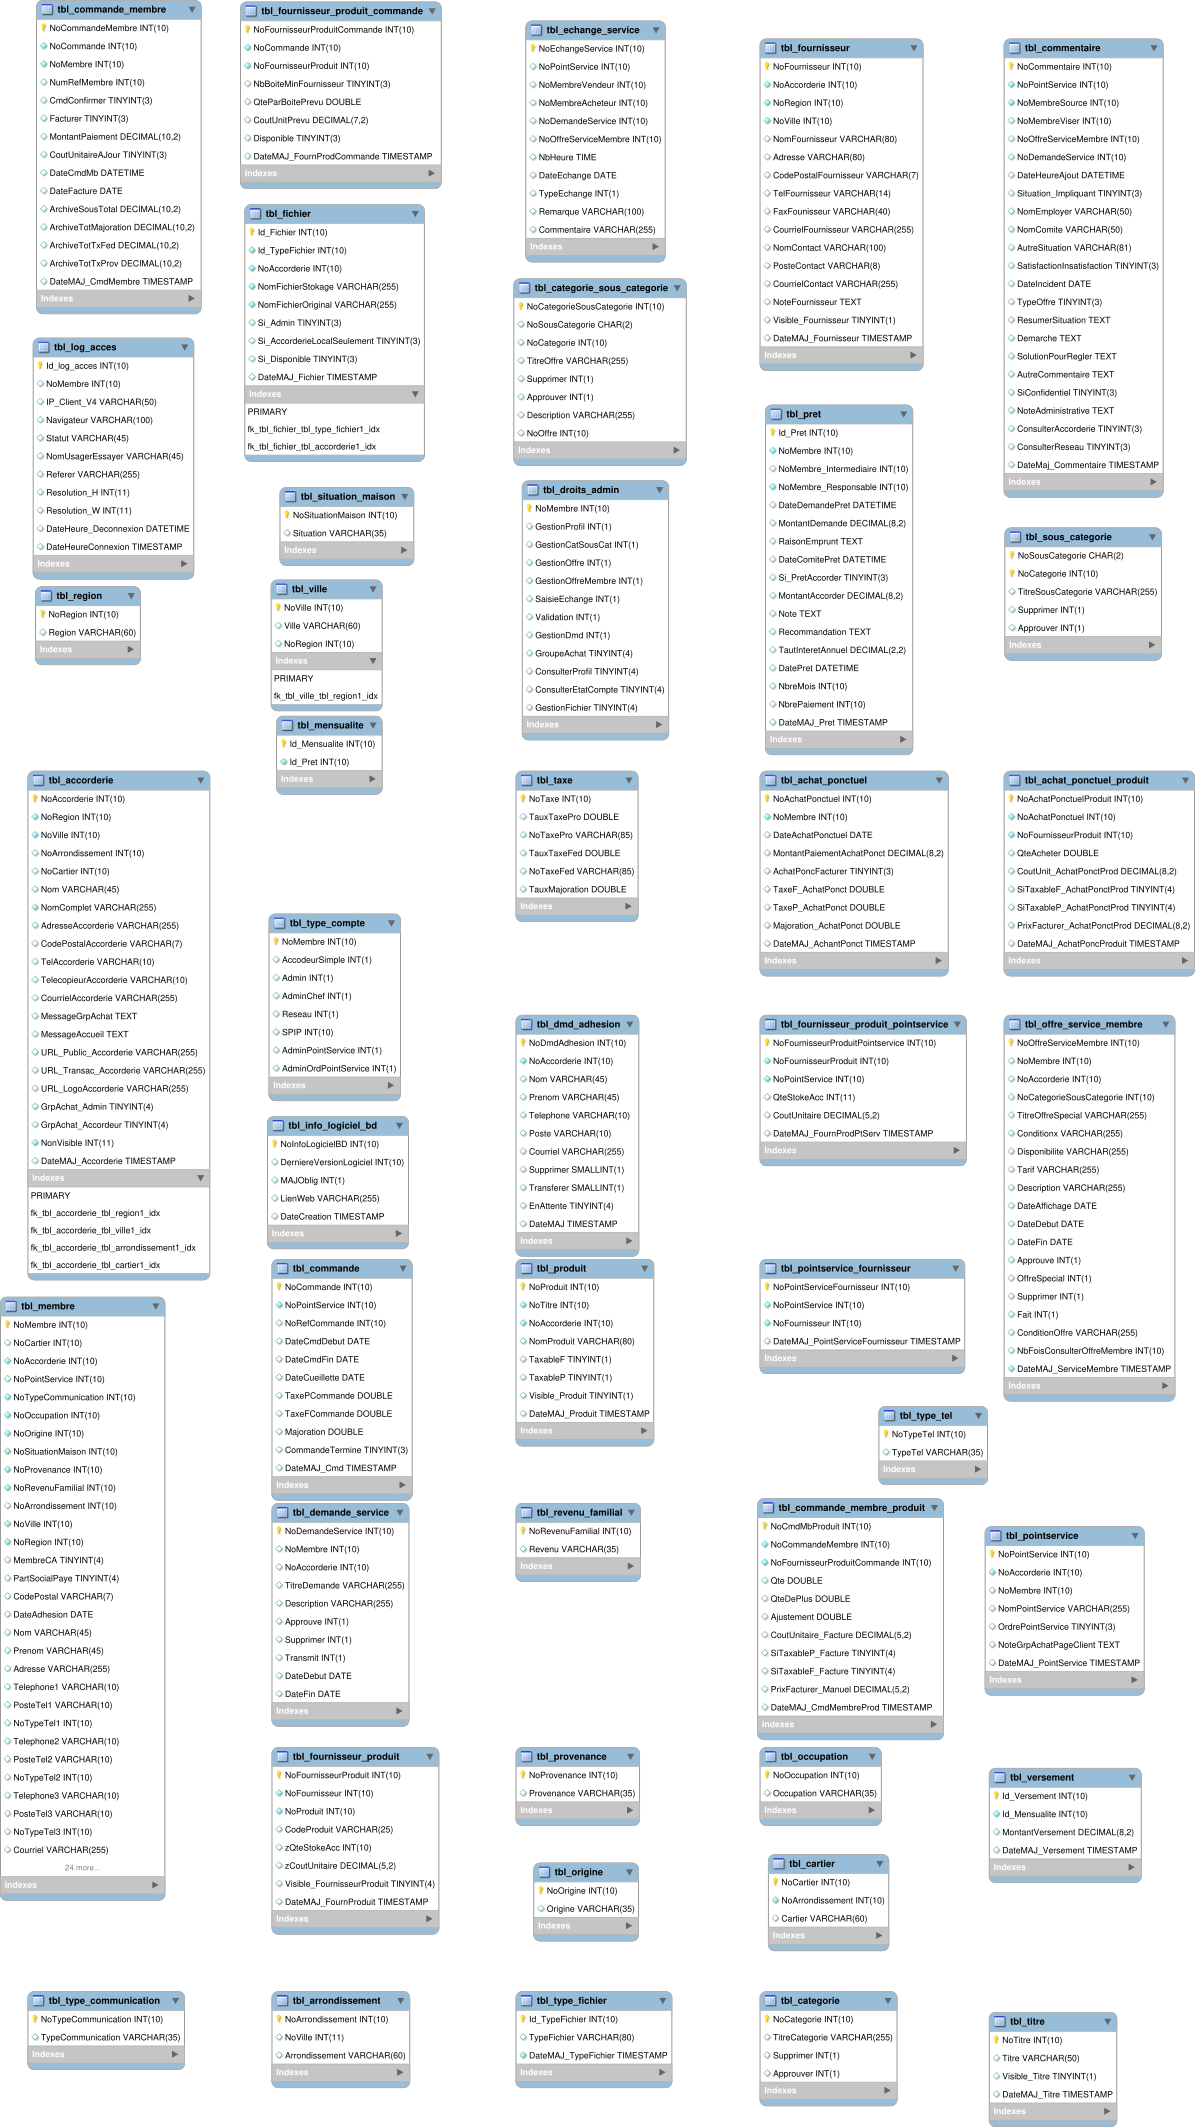
\includegraphics[height=7in]{schema_bd_accorderie.png}
\end{figure}

\Annexe{Diagramme nouveau modèle de données Espace Membre Accorderie 2023} \label{annexe_db_accorderie_2023}

\begin{figure}[htb]
\centering
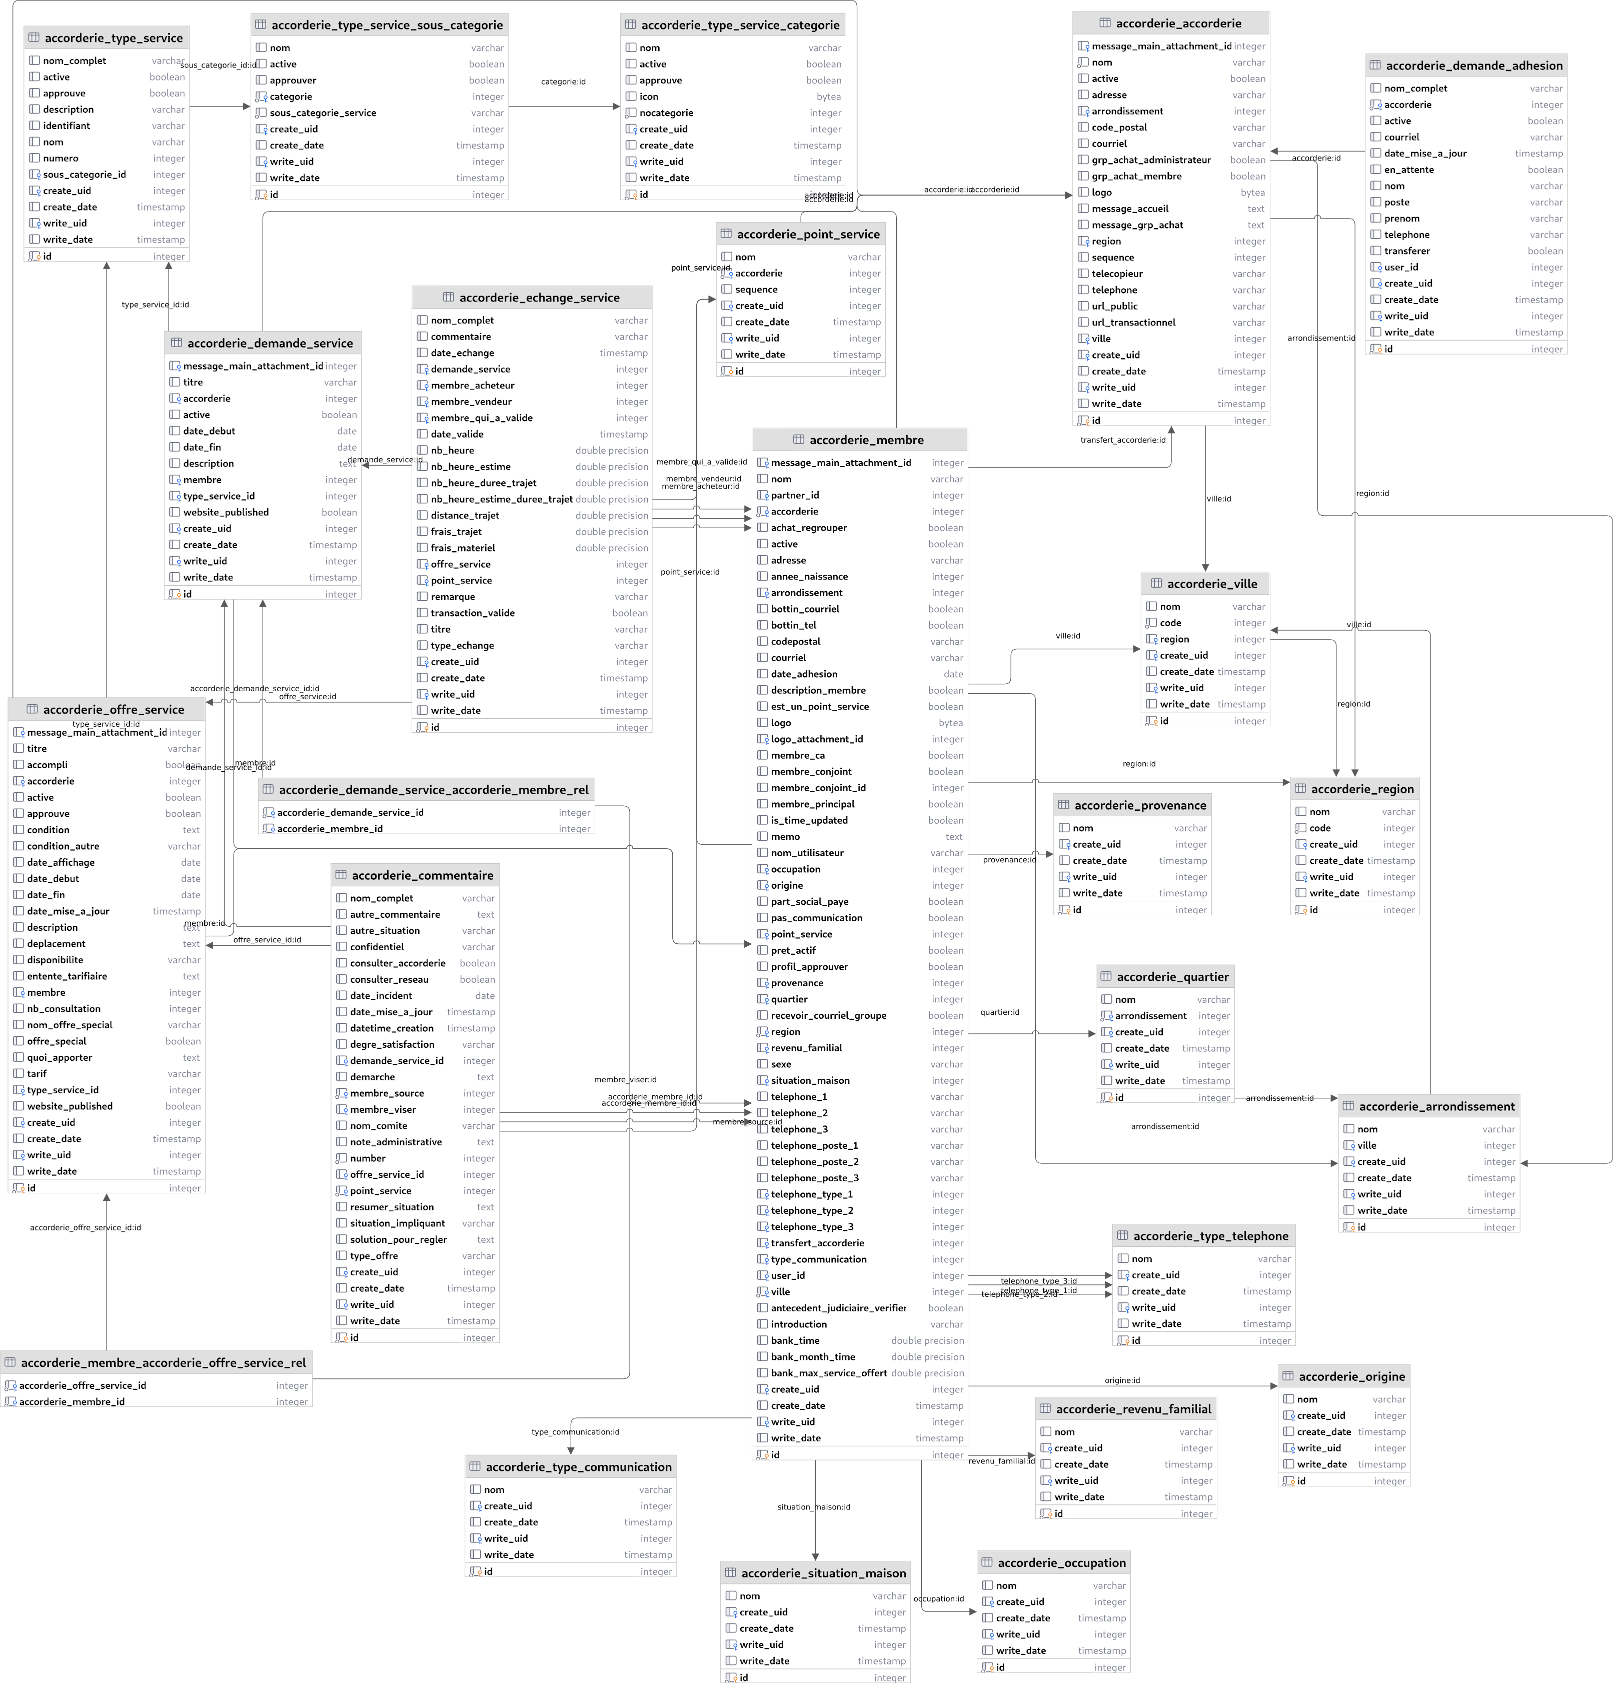
\includegraphics[width=\textwidth]{schema_bd_accorderie_new_small.png}
\end{figure}

\Annexe{Diagramme processus pour demander, offrir, établir un échange et le valider - Accorderie 2023} \label{annexe_processus_accorderie_2023}

\begin{figure}[htb]
\centering
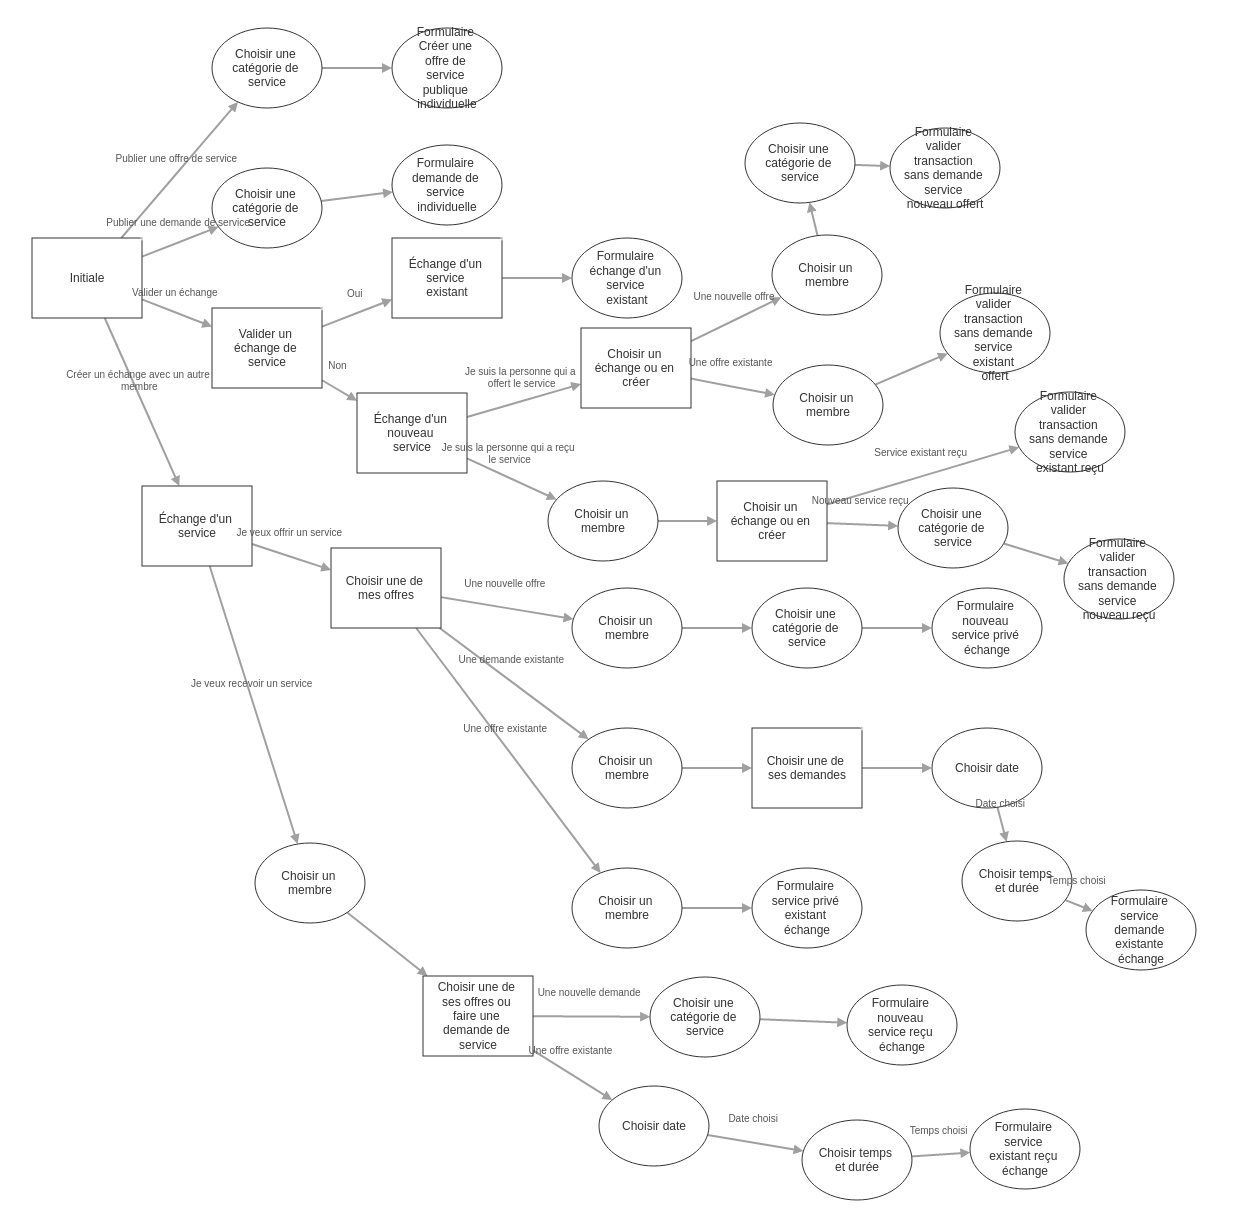
\includegraphics[width=\textwidth]{accorderie_processus.png}
\end{figure}

\Annexe{Diagramme modèle de données du portail CEPPP septembre 2022} \label{annexe_db_ceppp_2022}

\begin{figure}[htb]
\centering
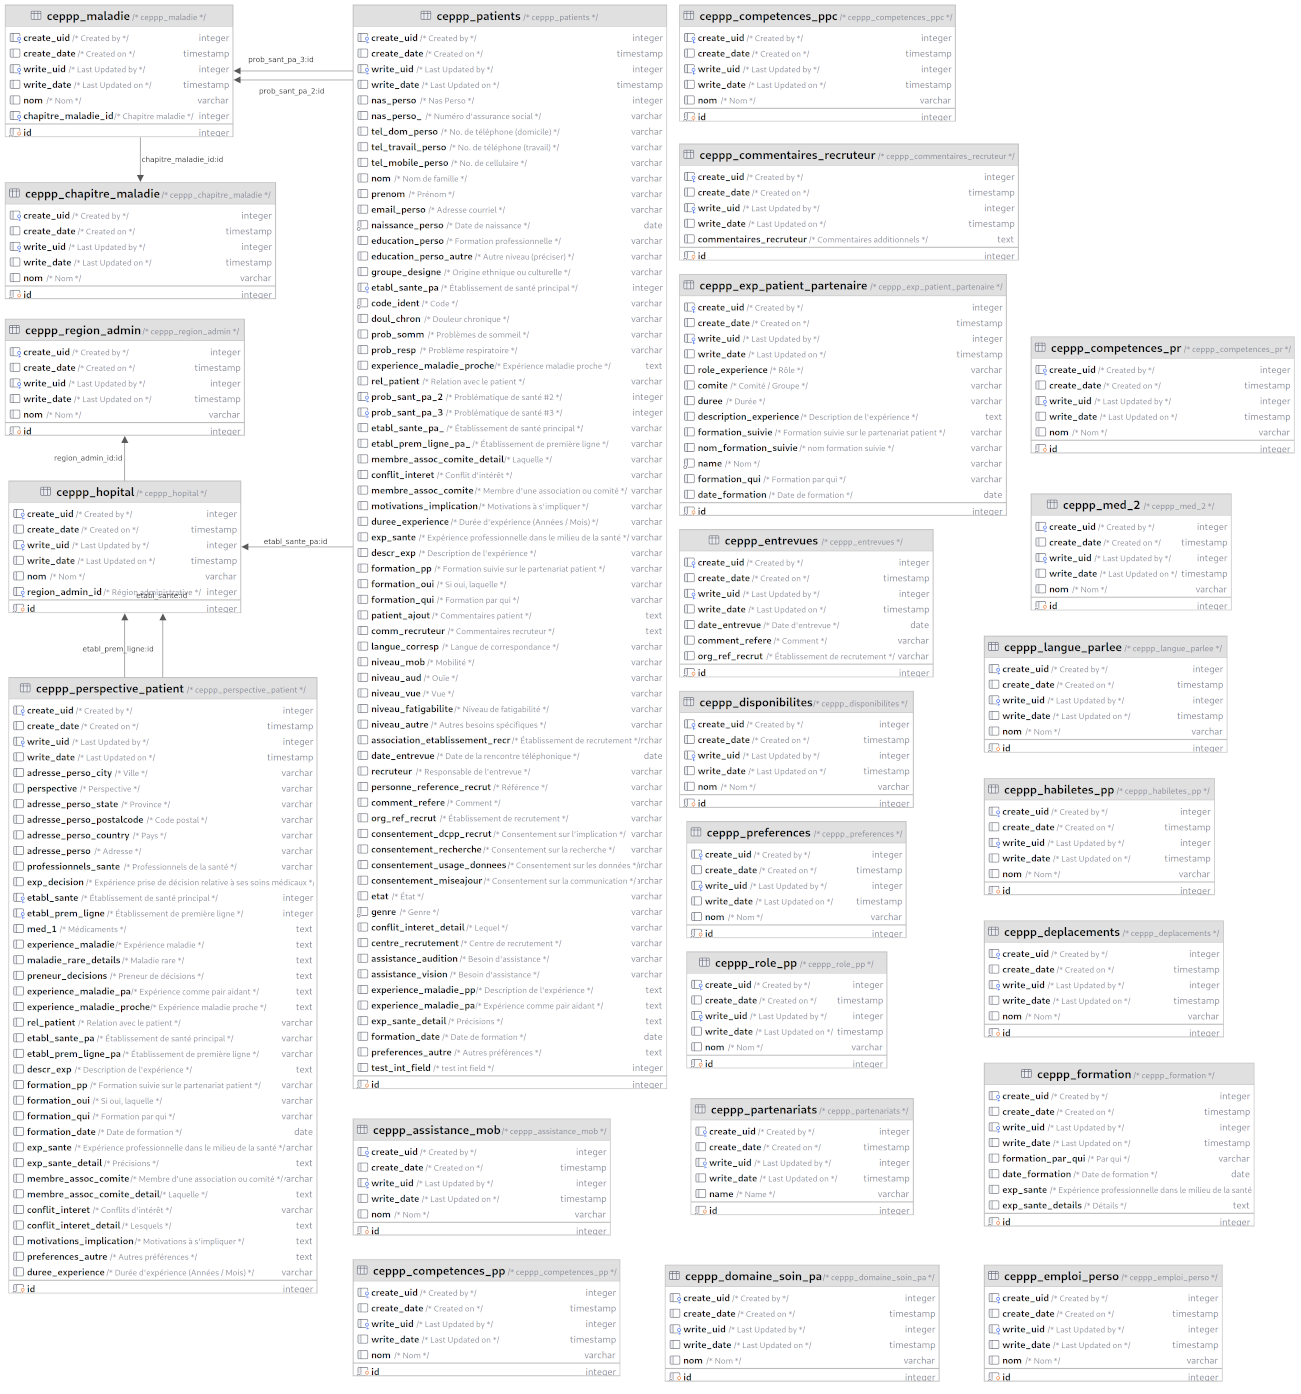
\includegraphics[width=\textwidth]{schema_bd_ceppp_suite_crm_small.png}
\end{figure}

\Annexe{Vue formulaire administration portail CEPPP} \label{annexe_form_ceppp_2022}

\begin{figure}[htb]
\centering
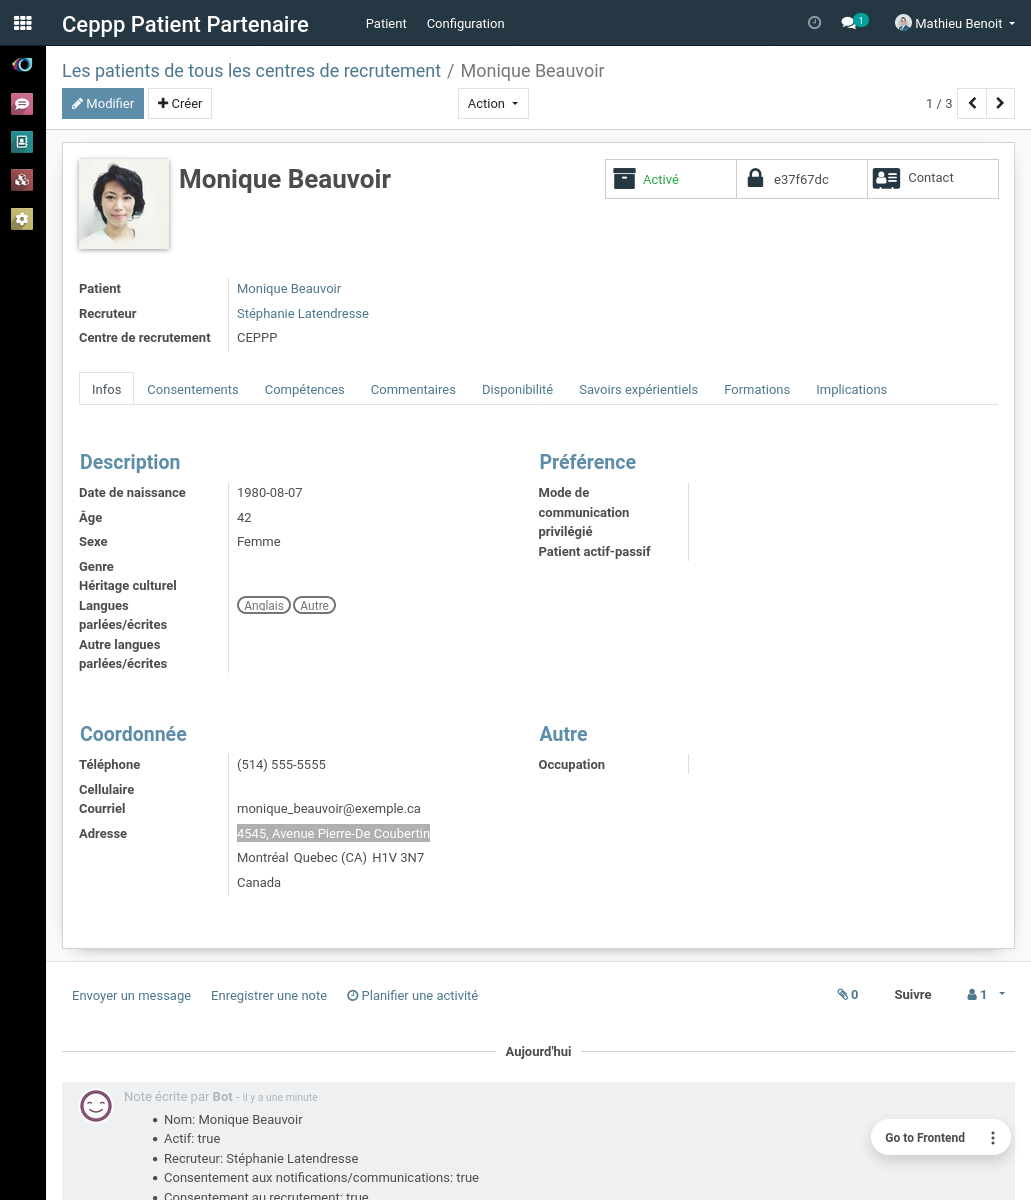
\includegraphics[height=7in]{exemple_vue_formulaire_patient_ceppp.png}
\end{figure}

\Annexe{Vue formulaire partenaire portail CEPPP} \label{annexe_form_anonyme_ceppp_2022}

\begin{figure}[htb]
\centering
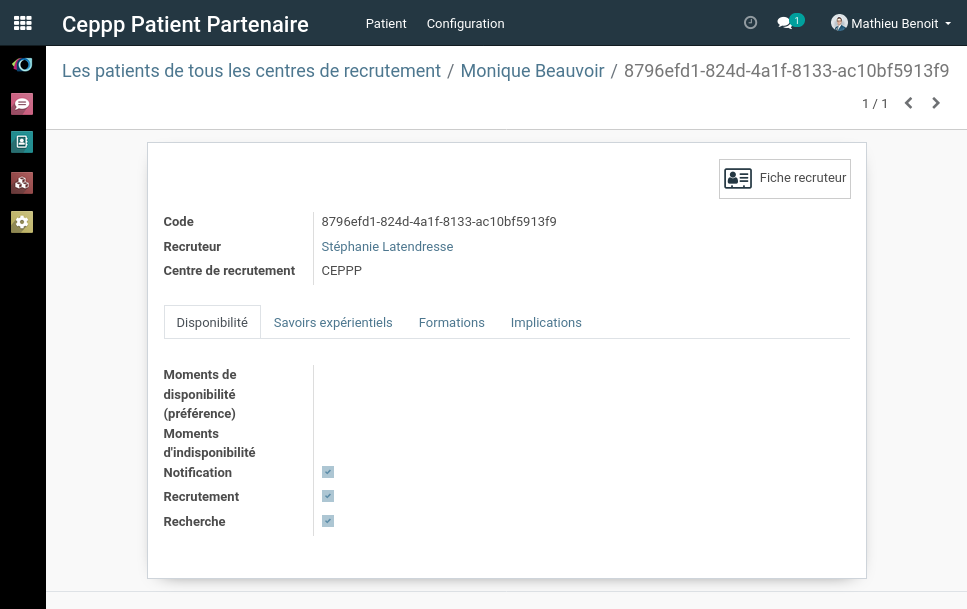
\includegraphics[width=\textwidth]{exemple_vue_formulaire_patient_anonyme_ceppp.png}
\end{figure}

% \Annexe{Analyse fonctionnelle portail CEPPP} \label{annexe_analyse_fonctionnelle_ceppp_2022}

% % \textbf{Analyse des besoins}


% \begin{table}[htb]
% \centering
% \begin{tblr}{
%   width = \linewidth,
%   colspec = {Q[110]Q[832]},
%   cell {1}{1} = tablegray,
%   cell {1}{2} = tablegray,
%   hlines,
%   vlines,
% }
% \textbf{Question}  & \textbf{Réponse}\\
% Définition & Le Portail des partenaires (“Portail”) du Centre d’excellence sur le partenariat avec les patients et le public (CEPPP) est issu de la fusion de communautés de patients partenaires, entre autres de la Direction collaboration et partenariat patient (DCPP) de la Faculté de médecine de l’Université de Montréal, et celle du CEPPP du Centre de recherche du Centre Hospitalier de l’Université de Montréal (CR-CHUM). Le Portail est un outil qui vient soutenir les activités de recrutement et de recherche sur les pratiques de partenariat.~ \\

% \end{tblr}
% \end{table}

\Annexe{Code u$_C^0$ dans le générateur de code} \label{annexe_cg_code_uc0}

\begin{lstlisting}[language=Python, upquote=true]
import os

from odoo import SUPERUSER_ID, _, api, fields, models

# TODO HUMAN: change my module_name to create a specific demo functionality
MODULE_NAME = "code_generator_demo"


def post_init_hook(cr, e):
   with api.Environment.manage():
       env = api.Environment(cr, SUPERUSER_ID, {})

       # The path of the actual file
       # path_module_generate = os.path.normpath(os.path.join(os.path.dirname(__file__), '..'))

       short_name = MODULE_NAME.replace("_", " ").title()

       # Add code generator
       value = {
           "shortdesc": short_name,
           "name": MODULE_NAME,
           "license": "AGPL-3",
           "author": "TechnoLibre",
           "website": "https://technolibre.ca",
           "application": True,
           "enable_sync_code": True,
           # "path_sync_code": path_module_generate,
       }

       # TODO HUMAN: enable your functionality to generate
       value["enable_template_code_generator_demo"] = True
       value["template_model_name"] = ""
       value["template_inherit_model_name"] = ""
       # value["template_module_path_generated_extension"] = "."
       value["enable_template_wizard_view"] = False
       value["force_generic_template_wizard_view"] = False
       value["disable_generate_access"] = False
       value["enable_template_website_snippet_view"] = False
       value["enable_sync_template"] = False
       value["ignore_fields"] = ""
       value["post_init_hook_show"] = True
       value["uninstall_hook_show"] = True
       value["post_init_hook_feature_code_generator"] = True
       value["uninstall_hook_feature_code_generator"] = True

       new_module_name = MODULE_NAME
       if (
           MODULE_NAME != "code_generator_demo"
           and "code_generator_" in MODULE_NAME
       ):
           if "code_generator_template" in MODULE_NAME:
               if value["enable_template_code_generator_demo"]:
                   new_module_name = f"code_generator_{MODULE_NAME[len('code_generator_template_'):]}"
               else:
                   new_module_name = MODULE_NAME[
                       len("code_generator_template_") :
                   ]
           else:
               new_module_name = MODULE_NAME[len("code_generator_") :]
           value["template_module_name"] = new_module_name
       value["hook_constant_code"] = f'MODULE_NAME = "{new_module_name}"'

       code_generator_id = env["code.generator.module"].create(value)

       # Add dependencies
       lst_depend_module = ["code_generator", "code_generator_hook"]
       code_generator_id.add_module_dependency(lst_depend_module)
       code_generator_id.add_module_dependency_template(lst_depend_module)
       # Generate module
       value = {"code_generator_ids": code_generator_id.ids}
       env["code.generator.writer"].create(value)


def uninstall_hook(cr, e):
   with api.Environment.manage():
       env = api.Environment(cr, SUPERUSER_ID, {})
       code_generator_id = env["code.generator.module"].search(
           [("name", "=", MODULE_NAME)]
       )
       if code_generator_id:
           code_generator_id.unlink()
\end{lstlisting}